\documentclass[hyperref={bookmarks=false},aspectratio=169]{beamer}
\usepackage[utf8]{inputenc}

\usepackage{multirow,rotating}
\usepackage{color}
\usepackage{hyperref}
\usepackage{tikz-cd}
\usepackage{array}
\usepackage{mathtools,nccmath}%
\usepackage{etoolbox, xparse} 
\usepackage[all]{xy}
\usepackage{lmodern}
\usepackage[scale=2]{ccicons}
\usepackage{transparent}
\usepackage{eso-pic}
\usetikzlibrary{matrix,decorations.pathreplacing}

\def\singR{\mathcal{X}_{R}}
\def\singRbar{\mathcal{\overline{X}}_{R}}

\newcommand*{\graybullet}{\textcolor{gray}{\textbullet}}
\newcommand*{\bluebullet}{\textcolor{blue}{\textbullet}}
\newcommand*{\redbullet}{\textcolor{red}{\textbullet}}

\hypersetup{bookmarks=true,unicode=true,pdftoolbar=true,pdfmenubar=true,
	pdffitwindow=false,pdfstartview={FitH},pdftitle={UMSSM},
	pdfauthor={O. Ozdal}, pdfsubject={CAP2017},
	pdfcreator={O. Ozdal},pdfproducer={O. Ozdal}, pdfkeywords={Non-minimal 
		supersymmetry}{Beyond the Standard Model Physics}{sneutrino dark matter},
	pdfnewwindow=true,colorlinks=true,
	linkcolor=,citecolor=magenta,filecolor=magenta,urlcolor=cyan}

%\setwatermark{
\includegraphics[height=8cm]{./figures/DD.png}}

\usebackgroundtemplate%
{%
   
{{\transparent{0.2}\hspace{10cm}
\includegraphics[height=8cm]{./figures/DD.png}}}
}
%....................................

\NewDocumentCommand{\tens}{t_}
{%
	\IfBooleanTF{#1}
	{\tensop}
	{\otimes}%
}
\NewDocumentCommand{\tensop}{m}
{%
	\mathbin{\mathop{\otimes}\displaylimits_{#1}}%
}

% ---------------  Define theme and color scheme  
\usetheme[sidebarleft]{Caltech}  % 3 options: minimal, sidebarleft, sidebarright


%\setbeamertemplate{footline}[frame number]

% Information on the title page---------------------------
\title[]
{\bfseries{ANALYSE STATIQUE POUR LA CLASSIFICATION DES PROCEDURES CANDIDATE A LA TASKIFICATION}}



\author[]
{ \textbf{Encadré par: Jean-Baptiste BESNARD}\\  \and Karim SMAIL \and Sofiane BOUZAHER\ \and Asma KREDDIA\ \and Atef DORAI }

\institute
{
   Master CHPS 
   \\ \url{https://github.com/Taskification/Taskification}
}


% logo of my university
\titlegraphic{
\includegraphics[width=2cm]{./figures/logo-uvsq.png}}
%------------------------------------------------------------

%------------------------------------------------------------
%The next block of commands puts the table of contents at the 
%beginning of each section and highlights the current section:

\AtBeginSection[]
{
  \begin{frame}
    \frametitle{PLAN}
    \tableofcontents[currentsection]
  \end{frame}
}
%------------------------------------------------------------


\begin{document}

%\addtobeamertemplate{footline}{\insertframenumber/\inserttotalframenumber}
% <--- change here

\addtobeamertemplate{footline}{ \hfill \raisebox{0.25cm}[0pt][0pt]{\insertframenumber/\inserttotalframenumber\hspace{2em}\raisebox{-4em}\null}}

\frame{\titlepage}  % Creates title page

%---------   table of contents after title page  ------------
\begin{frame}
\frametitle{PLAN}
\tableofcontents
\end{frame}
%---------------------------------------------------------

\section{INTRODUCTION}

%---------------------------------------------------------

\subsection{Compilateur?}

%---------------------------------------------------------

%----------------------------------------------------------

\begin{frame}
\frametitle{Compilateur?}

\vfill
\begin{center} 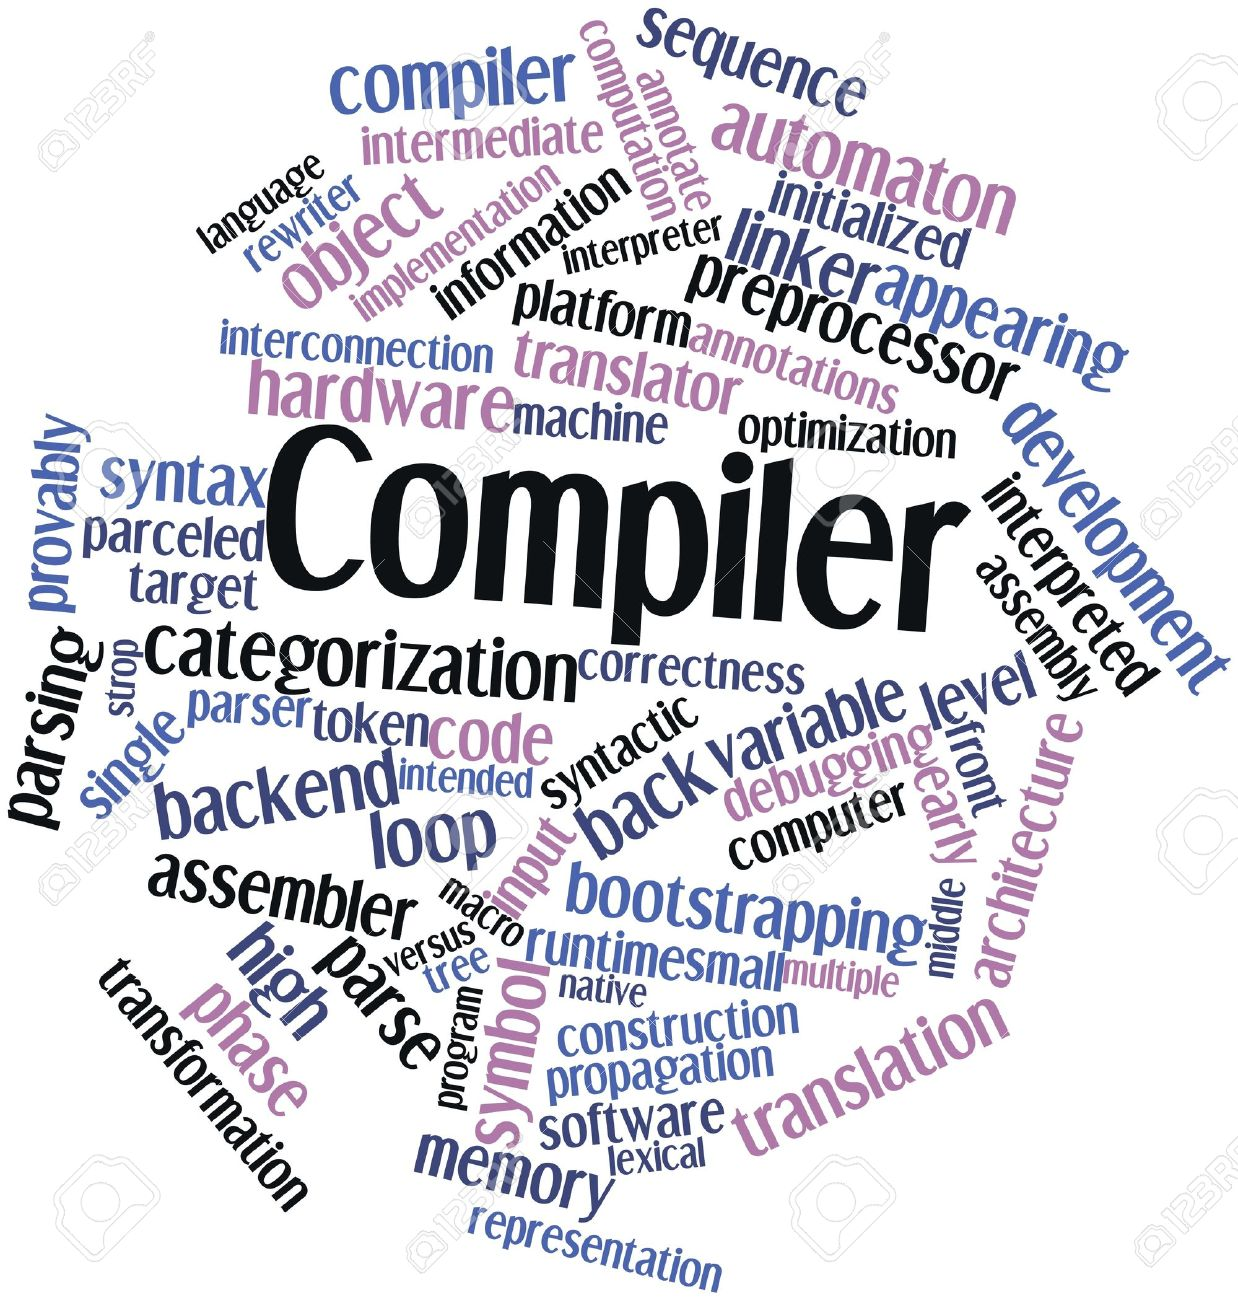
\includegraphics[scale=0.9]{./figures/COMPILATEUR.jpg} \\[1cm] \end{center}
\vfill


\end{frame}


%---------------------------------------------------------

\subsection{Malheureusement}


%---------------------------------------------------------

\begin{frame}
\frametitle{Malheureusement}

\vfill
\begin{center} 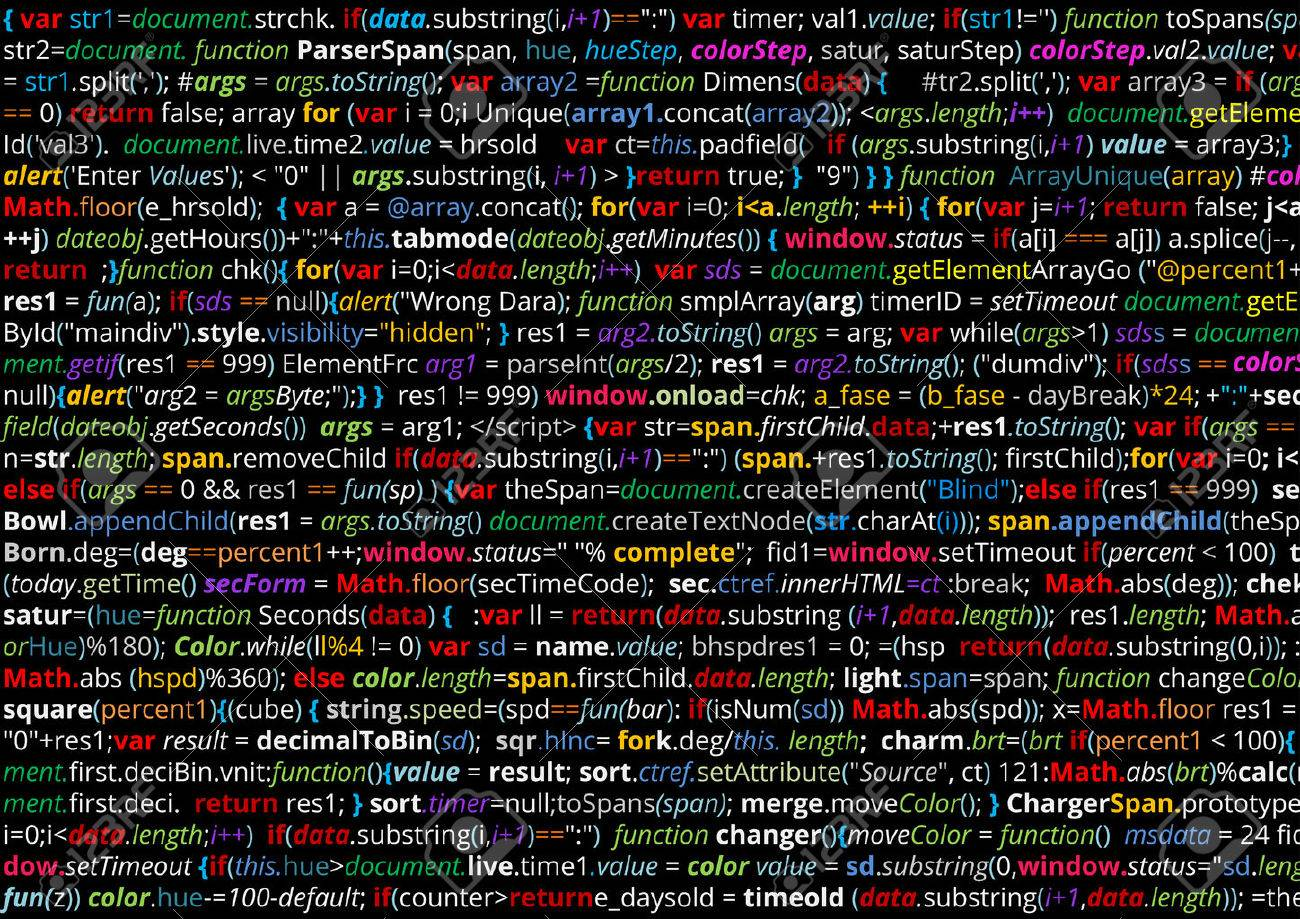
\includegraphics[scale=0.9]{./figures/pro.jpg} \\[1cm] \end{center}
\vfill

\end{frame}

%--------------------------------------------------------
\subsection{Laquelle}


%---------------------------------------------------------

\begin{frame}
\frametitle{Laquelle}

\vfill
\begin{center} 
\includegraphics[scale=0.6]{./figures/int.jpg} \\[1cm] \end{center}
\vfill

\end{frame}

%---------------------------------------------------------
%--------------------------------------------------------
\subsection{Plugin}


%---------------------------------------------------------

\begin{frame}
\frametitle{Plugin}
\begin{itemize}
    \item  \textbf{ Paquet qui Complète et apporte de nouvelles fonctionnalités pour le fameux "CLANG".}
\end{itemize}


\vfill
\begin{center} 
\includegraphics[scale=0.3]{./figures/pack.jpg} \\[2cm] \end{center}
\vfill


\end{frame}

%---------------------------------------------------------

\section{FONCTIONS PURES-IMPURES}

%---------------------------------------------------------
%---------------------------------------------------------

\subsection{Fonction pure}


%---------------------------------------------------------

\begin{frame}
\frametitle{Fonction pure}
\textbf{Une fonction est dite pure lorsque elle possède les propriétés suivantes :}
\begin{itemize}
    \item  \textbf{Sa valeur de retour ne varie pas avec les mêmes arguments.}
    \item \textbf{Son évaluation n'a pas d'effets de bord.}
\end{itemize}


\end{frame}

%--------------------------------------------------------
%---------------------------------------------------------

\subsection{Fonction impure}


%---------------------------------------------------------

\begin{frame}
\frametitle{Fonction impure}

\textbf{Une fonction est dite impure lorsque elle ne vérifie pas soit les deux propriétés, ou bien l'une des deux c'est à dire:}

\begin{itemize}
    \item  \textbf{Sa valeur de retour  varie.}
    \item \textbf{Son évaluation a un effet de bord.}
\end{itemize}

\end{frame}

%--------------------------------------------------------
\subsection{Question ?}


%---------------------------------------------------------

\begin{frame}
\frametitle{Question ?}

\vfill
\begin{center} 
\includegraphics[scale=0.7]{./figures/qst.png} \\[2cm] \end{center}
\vfill

\end{frame}

%--------------------------------------------------------
\subsection{Tout simplement}


%---------------------------------------------------------

\begin{frame}
\frametitle{Tout simplement}

\begin{itemize}
\item \textbf{Fiable pour construire des programmes complexe .}

\item \textbf{Prédictibles et donc facile a tester .}

\item \textbf{Facile a lire et aussi a debuger.}

\item \textbf{Réutilisable dans d'autres environnement. }

\item \textbf{Efficace pour le parallélisme .}
\end{itemize}





\end{frame}

%--------------------------------------------------------
%---------------------------------------------------------

\section{CLANG LLVM}

%---------------------------------------------------------

%---------------------------------------------------------

\begin{frame}
\frametitle{CLANG LLVM}

\begin{itemize}
    \item \textbf{le Frontend, les Passes, le backend}
\end{itemize}


\vfill
\begin{center} 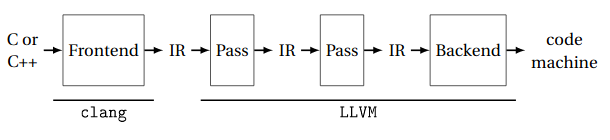
\includegraphics[scale=0.3]{./figures/ll.png} \end{center}
\vfill
\textbf{Plusieurs outils vont venir intervenir tels que :}\\[0.3cm]

\begin{itemize}
    \item CLANG
    \item OPT
    \item LLC
    \item LLVM-AS et LLVM-DIS
    \item LLI
\end{itemize}


\end{frame}

%--------------------------------------------------------
\section{AST}

%---------------------------------------------------------

\begin{frame}
\frametitle{AST(ABSTRACT SYNTAX TREE)}
\begin{itemize}
	\item \textbf{SYNTAX ?}
	\item \textbf{TREE ?}
	\item \textbf{ABSTRACT ?}	
    \item \textbf{Une représentation indispensable.}
    \item \textbf{Les compilateurs et la notion de L'AST.}
  %  \item \textbf{Une structure en C++ assez complexe de classes avec héritages.}
%    \item LLC
%    \item LLVM-AS et LLVM-DIS
 %   \item LLI
\end{itemize}
  

\end{frame}
%--------------------------------------------------------
\subsection{Exemple}

%---------------------------------------------------------

\begin{frame}
\frametitle{Exemple de l'AST}
\begin{itemize}
	\item \textbf{Code source :}
\end{itemize}
\vfill
\begin{center} 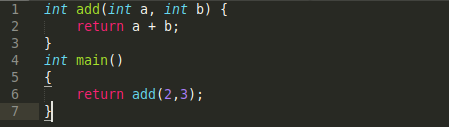
\includegraphics[scale=0.3]{./figures/add.png}  \end{center}
\vfill
\begin{itemize}
	\item \textbf{L'AST correspondant :}
\end{itemize}  
\vfill
\begin{center} 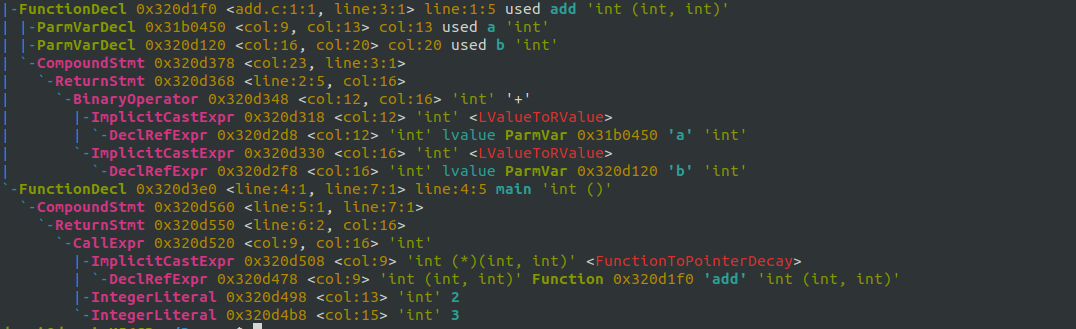
\includegraphics[scale=0.4]{./figures/ast.png} \end{center}
\vfill

\end{frame}
%--------------------------------------------------------
\section{DESCRIPTION DU CODE}

%---------------------------------------------------------

\begin{frame}
\frametitle{Description du code}
\textbf{Le code de plugin est implémente en C++ ,et construit de trois classes :}
\begin{itemize}
  \item \textbf{Classe TaskVisitor}
\end{itemize}

\vfill
\begin{center} 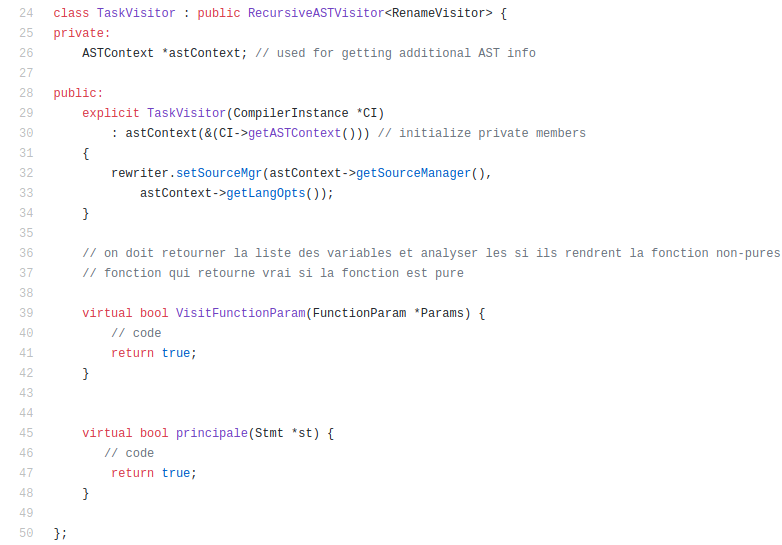
\includegraphics[scale=0.3]{./figures/class1.png} \\[2cm] \end{center}
\vfill



\end{frame}

%---------------------------------------------------------

\begin{frame}
\frametitle{Description du code}
\begin{itemize}
  \item \textbf{Classe TaskASTConsumer }
\end{itemize}
  \vfill
\begin{center} 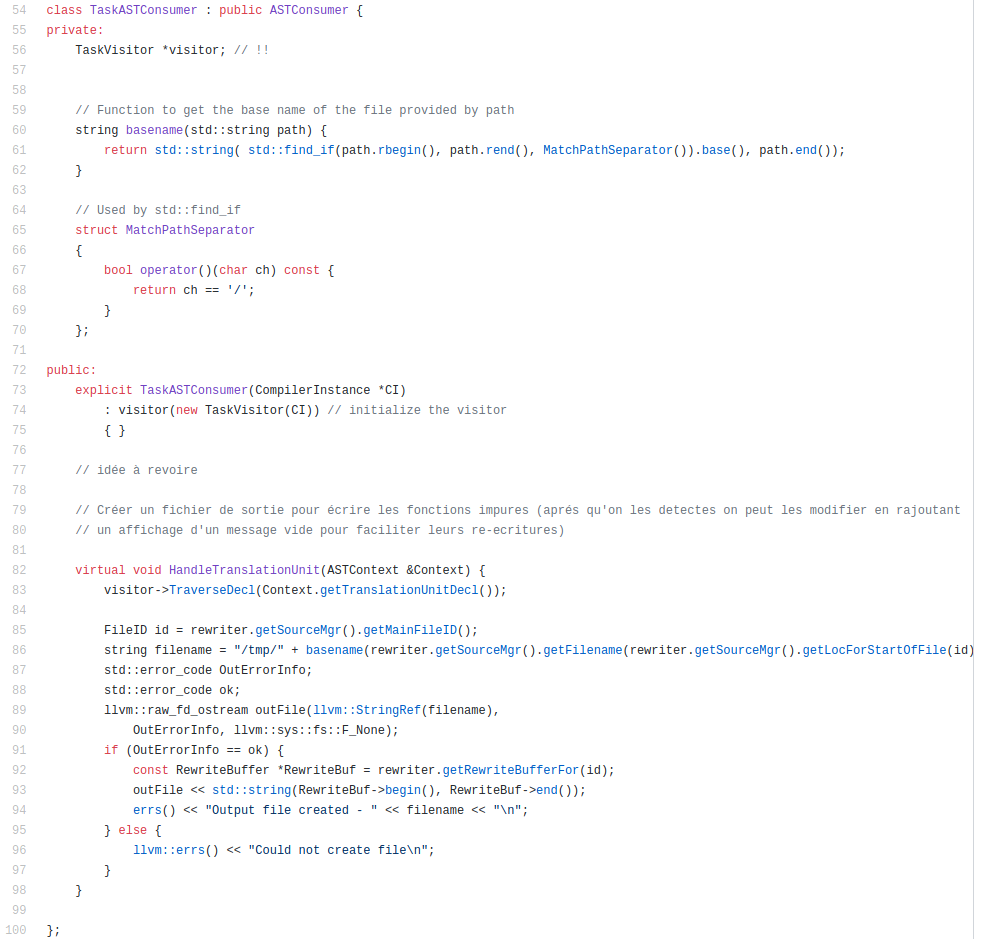
\includegraphics[scale=0.22]{./figures/class2.png} \\[2cm] \end{center}
\vfill



\end{frame}
%--------------------------------------------------------
\begin{frame}
\frametitle{Description du code}
\begin{itemize}
  \item \textbf{Classe PluginTaskAction}
\end{itemize}

\vfill
\begin{center} 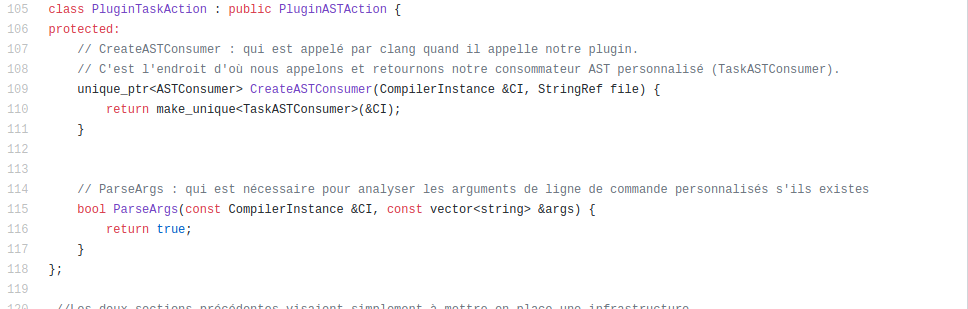
\includegraphics[scale=0.3]{./figures/class3.png}  \end{center}
\begin{itemize}
  \item \textbf{FrontendPluginRegistry}
\end{itemize}
\begin{center} 
\includegraphics[scale=0.3]{./figures/class4.png} \end{center}
\vfill




\end{frame}
%--------------------------------------------------------

%---------------------------------------------------------


\section{CONCLUSION}


\begin{frame}
\frametitle{Conclusion}

\begin{itemize}
 \item \textbf{Fonctions pures sont des fonctions qui offrent une grande stabilité et performance lors de l implémentation des programmes complexes comparément avec les fonctions impures .}
\item\textbf{Alimenter la chaîne de compilation CLANG-LLVM par de nouvelles fonctionnalités trace  le  point de départ pour rentrer dans le monde vaste des compilateurs. 
}
\item\textbf{Intégrer des plugins au compilateur  permet  d'améliorer leurs performances en jouant sur la mémoire réservée et le temps d'exécution.}
\item \textbf{Performance reste le mot clé  et le point d appui pour nous comme étant des ingénieurs HPC.
}
\end{itemize}


\end{frame}
%.........................................................
\begin{frame}

\vfill
\begin{center} 
\includegraphics[scale=0.7]{./figures/danke.jpg} \end{center}
\vfill

\end{frame}

%.........................................................

\end{document}